\newpage
\section{78. 子集}
\label{leetcode:78}

\subsection{题目}

给定一组\textbf{不含重复元素}的整数数组 nums,返回该数组所有可能的\textbf{子集}(\textbf{幂集})。

\textbf{说明}:解集不能包含重复的子集。

\textbf{示例}:

\begin{verbatim}
  输入: nums = [1,2,3]
  输出:
  [
    [3],
    [1],
    [2],
    [1,2,3],
    [1,3],
    [2,3],
    [1,2],
    []
  ]
\end{verbatim}

\subsection{参考题解}

如果 nums = [1,2,3],则状态树如下。其实这状态树都是想象出来的,
你递归的过程中,就好像是在树的节点之间移动一样。这样题目就比较好
理解了。这题则要求把树中的每一个节点都保存下来。

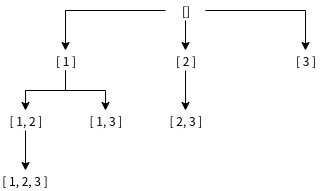
\includegraphics[width=100mm,height=70mm]{images/leetcode/leetcode_78.png}

\begin{verbatim}
/**
 * @param {number[]} nums
 * @return {number[][]}
 */
var subsets = function(nums) {
  let result = [];
  recursion(nums, 0, [], result);
  return result;
};

function recursion(nums, first, cur, result) {
  result.push(cur);
  for (let i = first; i < nums.length; i += 1) {
    recursion(nums, i + 1, cur.concat([nums[i]]), result);
  }
}
\end{verbatim}
